\subsection{PSYCHE pure shift NMR}
\label{subsec:poise__psyche}

In \cref{sec:pureshift__optimisation}, I described early attempts towards the optimisation of PSYCHE pure shift spectra.
The content in this section is similar, except that it was performed within the framework of POISE.

\begin{figure}[htb]
    \centering
    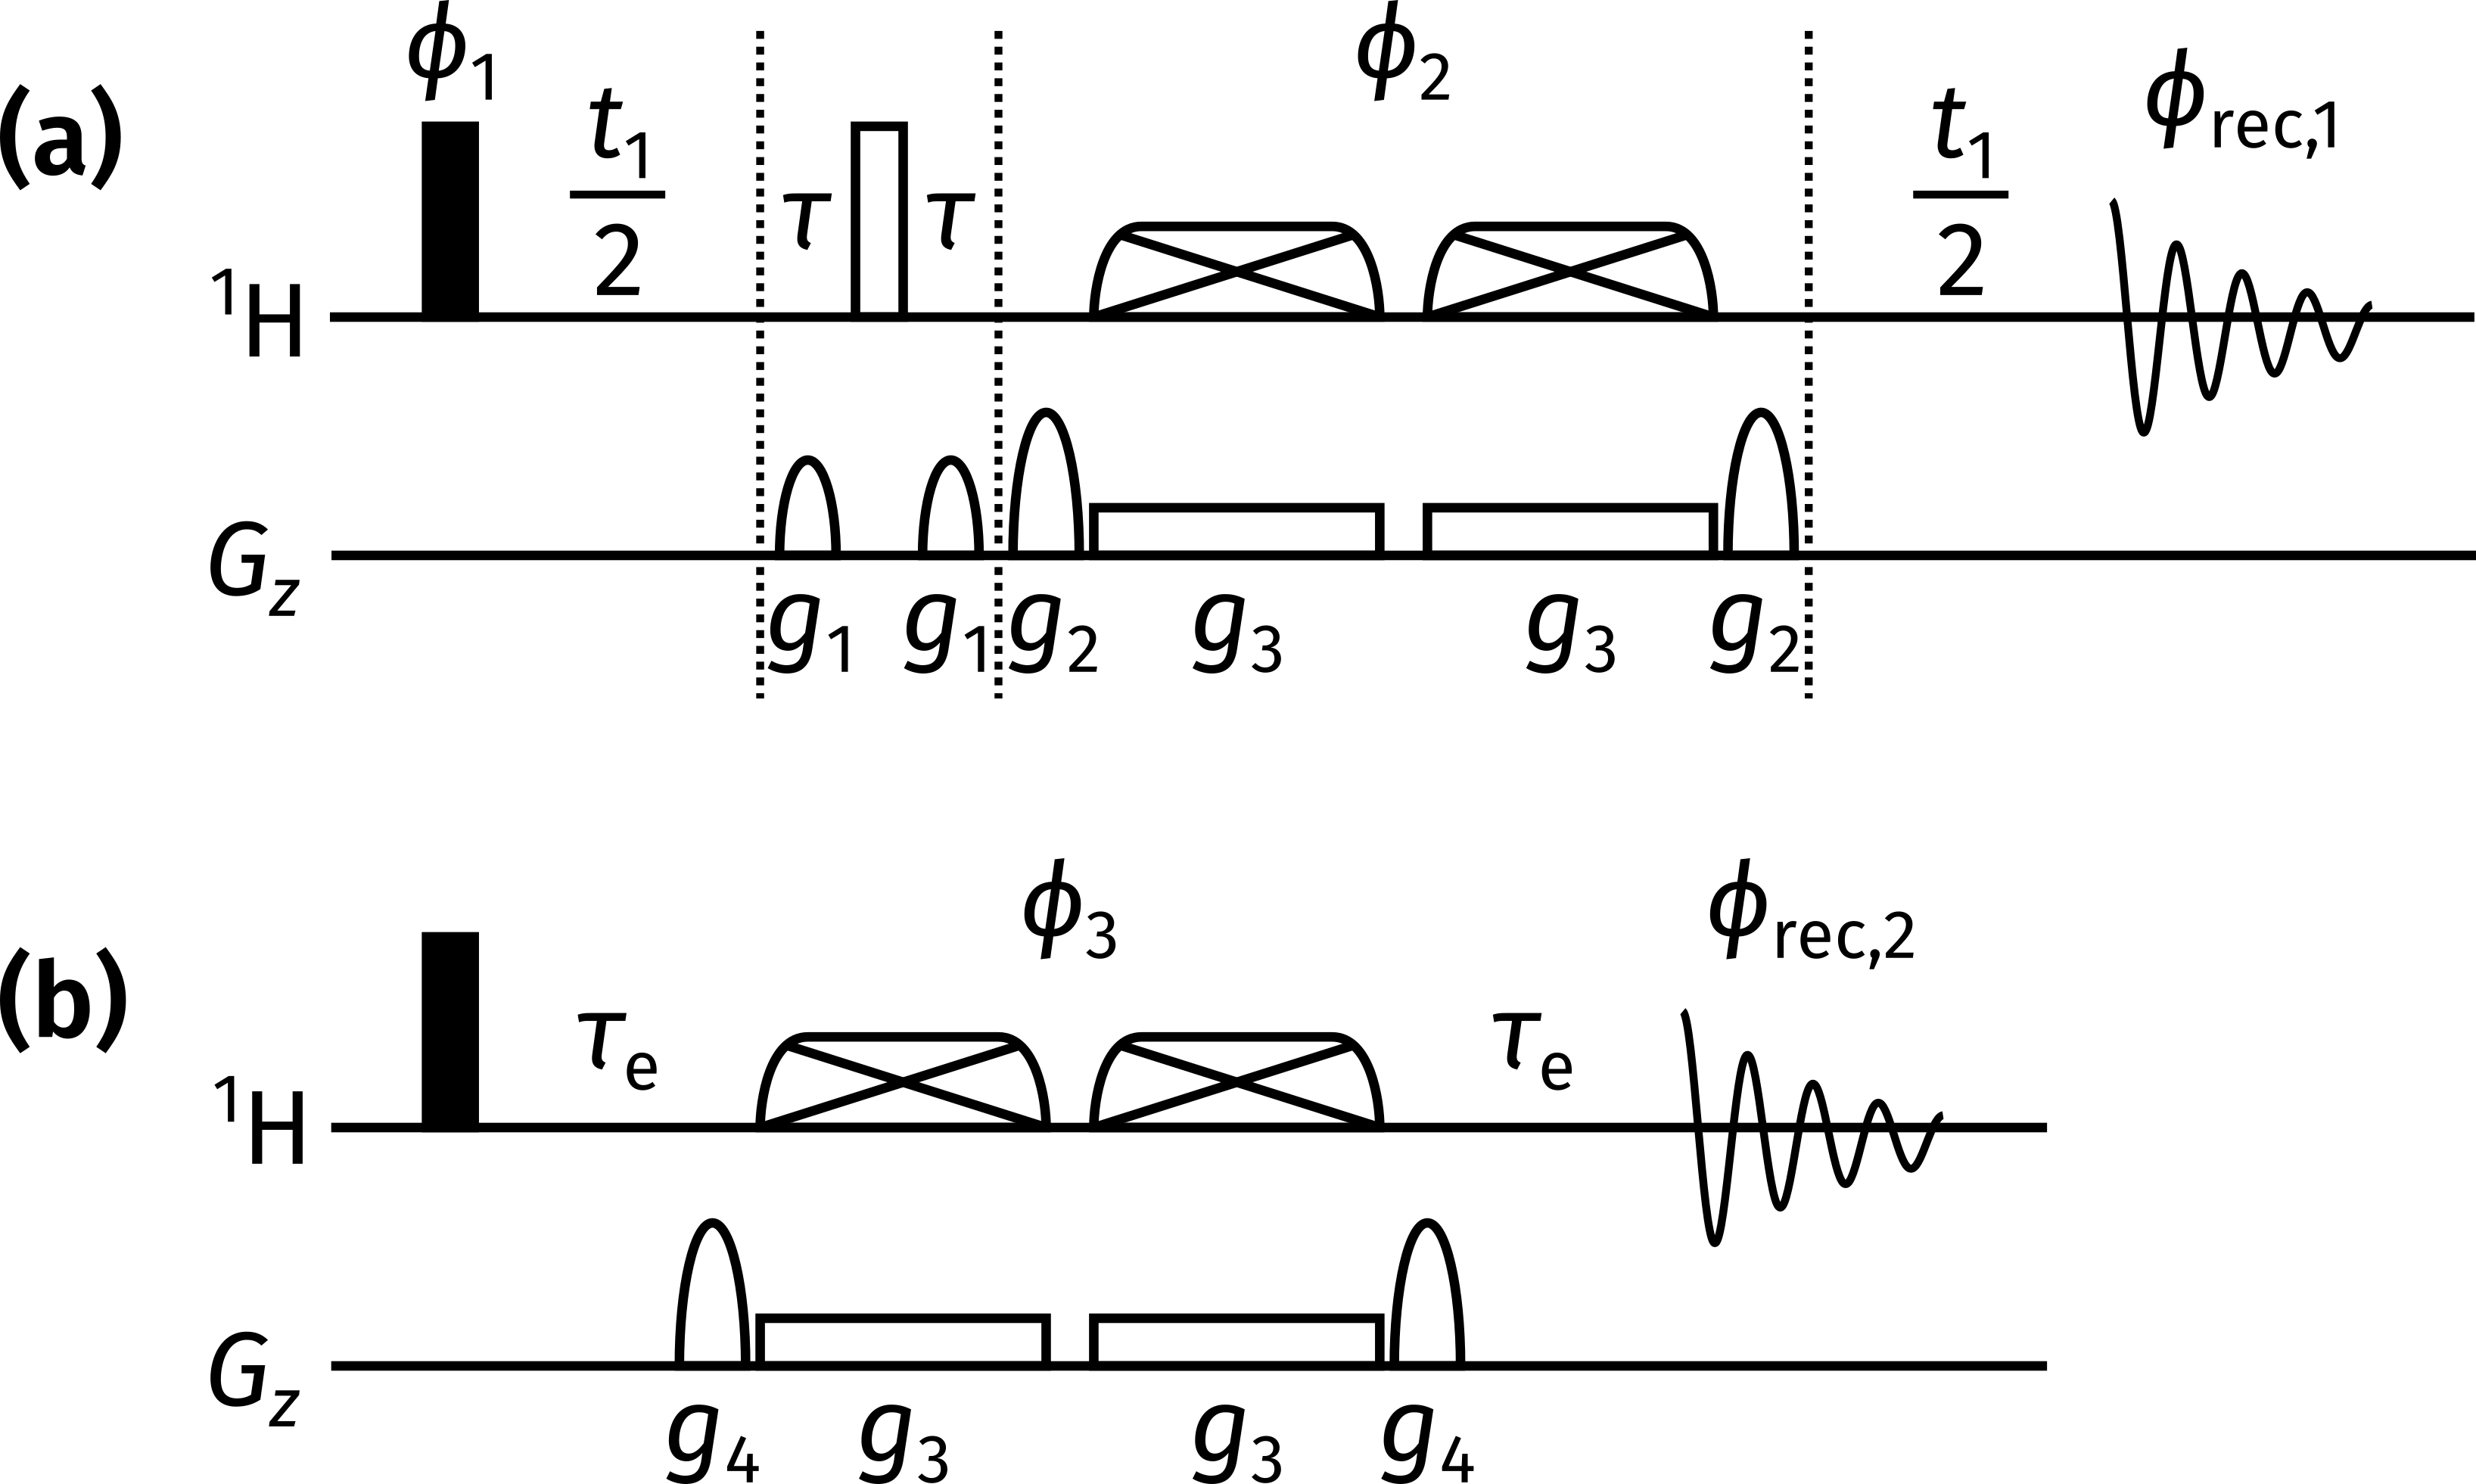
\includegraphics[]{pp/poise/psyche.png}
    {\phantomsubcaption\label{fig:poise_psyche_pulseq_psyche}}
    {\phantomsubcaption\label{fig:poise_psyche_pulseq_jrse}}
    \caption[Pulse sequences used for PSYCHE optimisations]{
        \textbf{(\subref{fig:poise_psyche_pulseq_psyche})} Pseudo-2D PSYCHE pure shift experiment.
        \textbf{(\subref{fig:poise_psyche_pulseq_jrse})} J-resolved spin echo experiment (see also \cref{subsec:pureshift__optim_techniques}) using the PSYCHE PSE.
        Phase cycling is performed using: $\phi_1 = (x, -x)$, $\phi_2 = (x, x, y, y)$, $\phi_{\text{rec},1} = (x, -x, -x, x)$ for the full PSYCHE experiment, and $\phi_3 = (x, y, -x, -y)$, $\phi_{\text{rec},2} = (x, -x, x, -x)$ for the JRSE experiment.
        Gradient amplitudes are $(g_1, g_2, g_3, g_4) = (35\%, 77\%, 2\%, 50\%)$ (though the exact value of the CTP gradients are likely immaterial).
        The delay $\tau$ is set to $1/(4 \cdot T_\text{chunk})$ for the PSYCHE experiment, and $\tau_\text{e}$ is \SI{16}{\ms}.
    }
    \label{fig:poise_psyche_pulseq}
\end{figure}



\subsubsection{Optimisation setup}

In this section, the standard double-saltire PSYCHE pure shift element was used (\cref{fig:poise_psyche_pulseq_psyche}).
As described in \cref{subsec:pureshift__optim_techniques}, the PSYCHE pure shift element can be described using six parameters; in this section, we investigate only three of these, namely the amplitude (i.e.\ flip angle), bandwidth, and duration.
In addition to this, the amplitude of the weak gradient during the PSE was also chosen as a fourth parameter to vary.
As before, the quality of the PSE is evaluated using a JRSE experiment (\cref{fig:poise_psyche_pulseq_jrse}), which is then compared against a pulse--acquire spectrum: the cost function used is $f_\text{diff}$.
In general, the spectral region being evaluated has to be appropriately chosen to exclude strong singlets, which are irrelevant to pure shift NMR but disproportionately influence the value of the cost function.

